%************************************************
\chapter{Building a Theory for Smart Stormwater Systems}\label{ch:theory}
%************************************************
\vspace{1cm}

\section{Introduction}

Rapid advances in sensing, computation, and wireless communications are promising to merge the physical with the virtual.
Calls to build the ``smart'' city of the future are being embraced by decision makers.
While the onset of self-driving cars provides a good example that this vision is becoming a reality, the role  of information technology in the water sector has yet to be fleshed out.
These technologies stand to enable a leap in innovation in the distributed treatment of urban runoff, one of ourlargest environmental challenges. 

\

Retrofitting stormwater systems with sensors and controllers will allow the city to be controlled in real-time as a distributed treatment plant.
Unlike static infrastructure, which cannot adapt its operation to individual storms or changing land uses, ``smart'' stormwater systems will use system-level coordination to reduce flooding and maximize watershed pollutant removal. Given the sheer number of storm water control measures in United States, even a small improvement to their performance could lead to a substantial reduction in pollutant loads.
Intriguingly, such a vision is not limited by technology, which has matured to the point at which it can be ubiquitously deployed. 
Rather, the challenge is much more fundamental and rooted in a system-level understanding of environmental science.
Once stormwater systems become highly instrumented and controlled, how should they actually be operated to achieve desired watershed outcomes?
The answer to this question demands the development of a theoretical framework for smart stormwater systems. 
In this chapter we lay out the requirements for such a theory.
Acknowledging that the broad adoption these systems may still be years away,  we also present and evaluate a modeling framework to allow for the simulation of smart stormwater systems before they become common place. 
Recent urban floods~\cite{Frosch2016}, many of which are driven by flashy events and inadequately sized infrastructure, are all too common example that aging stormwater infrastructure is struggling to keep pace with a dynamic and changing climate. 
While flood control often emerges as one of the most promising application areas, to illustrate the flexibility of smart stormwater systems this chapter will focus on the impacts to urban water quality.


\section{Do best local practices achieve the best global outcomes?}

Pollutants in runoff are threatening the health of downstream ecosystems, as evinced by harmful algal blooms, such as those on Lake Erie~\cite{Michalak2013Record-settingConditions} and the Chesapeake Bay~\cite{powledge2005chesapeake,Boesch2001ChesapeakeAgriculture}.
Simultaneously, ``dry'' regions of the country are struggling to find new and clean sources of water.
By some estimates, the capture of stormwater in Los Angeles~\cite{Geosyntec2014} and San Francisco~\cite{Garrison2014StormwaterCalifornia} could offset the water used by these cities.
This, however, requires at least some level of treatment to ensure that captured stormwater is safe for direct use or aquifer injection.
In the face of these challenges, novel solutions for stormwater management are needed.

\

Reductions in hydraulic or pollutant loads are commonly achieved via a set of distributed stormwater solutions~\cite{Hamel2013Source-controlReview, Burns2012HydrologicReform}, such as ponds or treatment wetlands.
Our body of knowledge on the treatment potential of these systems is extensive, showing that significant water quality and hydraulic benefits can be achieved at the level of individual sites~\cite{Stanley1996PollutantPond,Carleton2000PerformanceRunoff}.
Most recently, an exciting and growing research area has formed around smaller-scale and more distributed Green Infrastructure (GI) solutions, such as green roofs or bioswales\cite{Benedict2006GreenCentury}.
Most of these solutions are grouped under the broader umbrella of Best Management Practices\cite{Urbonas1994ASSESSMENTTECHNOLOGY} (BMPs) or Storm Water Control Measures (SCMs)\cite{Cizek201340}.

\

Given the aggressive adoption of these stormwater practices, rarely is the question asked: Does doing the ``best'' at a local scale translate to doing the best at the watershed scale? Research on this question is limited\cite{Petrucci2013DoOutcomes,Sage2015StormwaterPractices,Petrucci2014UrbanHow}, but paints a cautionary picture.
Unless designed as part of a coordinated, city-scale solution, a system of SCMs may actually worsen watershed-scale outcomes.
For example, unless coordinated at design-time, hydrographs from individual SCMs
may add up to cause larger downstream flows compared to the same watershed
without these SCMs\cite{Emerson2005Watershed-ScaleBasins}.
This, in turn, can lead to increased stream erosion and re-suspension of sediment-bound pollutants.
More examples can be given, but there is an urgent need to investigate the
scalability of SCMs and to ensure that their functionality is tuned in the context of the broader stormwater system. 

\

Even if system-level optimization is used to determine the placement of SCMs\cite{Ciou2012OptimizationWatershed,Zhen2004OptimalScale}, it is difficult to guarantee that the overall system will perform as designed.
The sheer variability in rainfall\cite{Chaubey1999UncertaintyRainfall}, seasonal pollutant loadings\cite{Ouyang2006AssessmentQuality}, and broader land use changes\cite{Goonetilleke2005UnderstandingManagement} will always push stormwater systems beyond their intended design or the ``average'' storm\cite{DepartmentofEnvironmentalProtection2006PennsylvaniaManual}.
As such, it becomes imperative to find a way to adapt to these uncertain disturbances.
One solution relies on real-time sensing and control.
By equipping stormwater elements with control valves, which can be operated in real-time based on sensor readings, the overall performance of the entire system can be adapted to achieve watershed-scale benefits (Figure.\ref{fig-ch1:vision}a). 

%%------------------RTC studies ---------------
\subsection{Existing studies on real-time control}

The bulk of existing literature on real-time control of stormwater SCMs focuses on water quality and hydraulic impacts at individual sites, particularly ponds and basins.
These studies assume that the outlet of a BMP has been retrofitted with a remotely controllable gate or valve.
By strategically controlling outflows before or during storm events, internal volumes can be modified and hydraulic retention time (HRT) can be increased.
Jacopin et al.\cite{Jacopin2001OptimisationBasins} demonstrated that detention basins, designed for flood control, can reduce sediment-based pollutant loading (57\% decrease) in downstream water bodies by simply opening and closing a valve.
Middleton et al.\cite{Middleton_2008} analyzed the water quality response of a controlled detention basin, observing up to a 90\% improvement in TSS and ammonia-nitrate removal.
Recent studies\cite{Muschalla2014Ecohydraulic-drivenBasins,
  Gaborit2013ImprovingForecasts,Gaborit2016} in Quebec, Canada,
proposed a rule-based control logic for a pond, based on rainfall forecasts, to
maximize retention time and  reduce hydraulic shocks to the downstream water
bodies. The authors observed a 90\% improvement in TSS retention. A
comprehensive review of these and other studies is summarized in Kerkez et al.\cite{kerkez2016}, along with additional information on how these solutions are deployed in the field. 
While these studies demonstrate significant potential to improve water quality at the scale of individual sites, the mechanisms behind the removal of pollutants in controlled SCMs remain a research challenge. This is particularly true in the removal of dissolved pollutants, such as ammonia and nitrate. Furthermore, the scalability of  real-time control must be evaluated to ensure that local benefits do not overshadow watershed-scale benefits. 

\

\begin{figure}
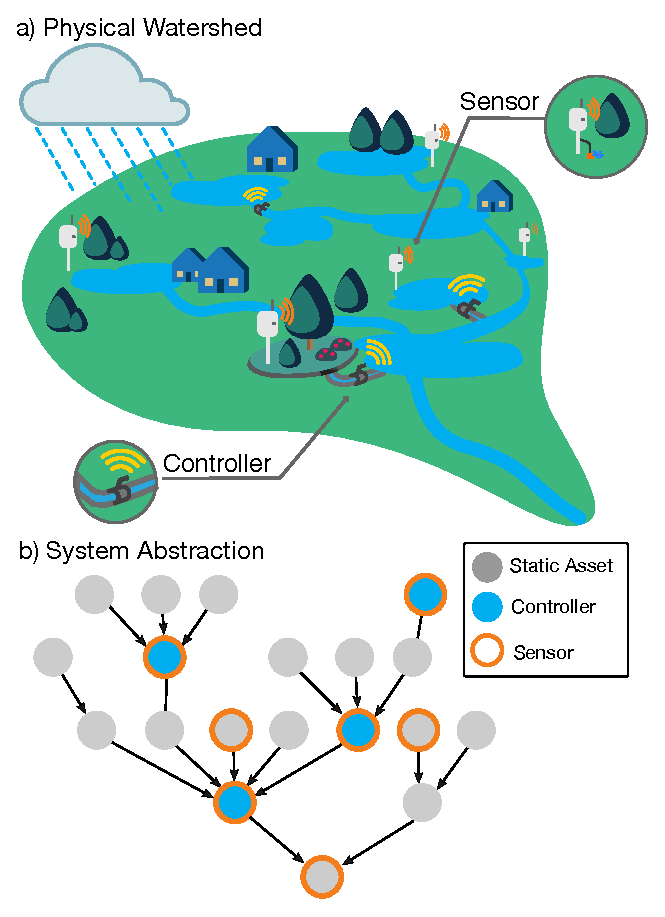
\includegraphics{gfx/Chapter-1/k-drawing.eps} 
\caption{Application of control and optimization methods to the real-time operation of stormwater systems will be made possible by abstracting physical models to system-theoretic representations.}\label{fig-ch1:vision}
\end{figure}


Since the 2000 European Union's Water Framework Directive~\cite{TheEuropeanParliamentandthecouncilofEuropeanUnion2000DirectivePolicy} there has been an increasing emphasis on integrated, system-level control of sewer water distribution systems.
The resulting control strategies vary in complexity\cite{Benedetti2009AScale,Seggelke2013ImplementationWilhelmshaven,Fiorelli2013OptimisedFunction}  and have since been implemented in a number of urban water networks\cite{Mollerup2016}.
Applying these methods to distributed stormwater solutions introduces a new set of challenges, however. Unlike in well-maintained sewer networks, the exposed and distributed  nature of stormwater systems introduces complexities associated with the urban hydrologic cycle, such as infiltration, evaporation, soil moisture and groundwater dynamics. Furthermore, one major function of stormwater systems relates to the  distributed control of  a large variety of solid, dissolved and emerging pollutants. Control of sewer networks is often targeted at volume control to mitigate sewer overflows or overloading treatment plants. As such, much work remains to be conducted on investigating how these methods can be applied to the distributed control of SCMs. 



\section{Toward a framework for smart stormwater systems}
 
Many methods have been developed by the operational research and control theory communities to optimize the operation of networked systems\cite{Sheffi1984UrbanNetworks,Astrom2006FeedbackEngineers}. Given their inherent non-linearity and complexity, existing stormwater models are not compatible with these tools. To that end, our knowledge of treatment processes and the physical nature of stormwater systems must first be embedded in a system-theoretic framework (Figure.\ref{fig-ch1:vision}b). Such a formal and mathematical approach will be crucial toward developing a system-level understanding of stormwater. Not only will this framework help to control future stormwater systems, but it will also create a foundation upon which to answer critical questions, such as: How many controllers are needed and where should they be placed to achieve best system-level benefits?  Consequently, how many sensors are needed and where should they be placed to help the control system achieve these objectives? 

\

Until sensors and controllers become ubiquitously deployed across stormwater systems, which may take years to accomplish, there is enough domain knowledge embedded in existing models to begin answering these questions through simulation. 


%%simulation framework
\subsection{Limitations of existing simulations approaches}
Existing stormwater models can be broadly grouped into two categories: those
that focus on hydrology (including hydraulics) and those that focus on water quality. The former range across simple routines, such as Muskingum routing\cite{Brunner1991ANetworks} and the Rational Method\cite{Chin2000Water-resourcesEngineering}, to more complex hydrodynamic models that solve the St.Venant's equation, such as popular packages like SWMM\cite{Rossman2010Storm5.1} and HEC-RAS\cite{Brunner2016HECManual}. The latter, which include models such as HYDRUS\cite{Rizzo2014ModellingHYDRUS-CWM1,Palfy2014TheData} and FITOVERT\cite{Giraldi2010FITOVERT:Wetlands},  are used to simulate treatment processes within individual sites, such as wetlands and green infrastructure. The coupling of the two approaches often yields  
While some packages support extended features that model both hydrology and
storm water quality, much work needs to be conducted to improve their
accuracy. This often forces a trade-off between
comprehensively modeling system-level hydrology or local-level treatment.

\

Pollutant removal in stormwater is a highly complex and dynamic process. The rate at which pollutants undergo transformation is dependent upon the pollutant-type and its interaction with a given stormwater element (oxygen concentrations, soil types, biomass, settling times, water temperature, etc). Given the complexity of these interactions, popular hydraulic models, such as SWMM, MUSIC\cite{Wong2002AConceptualisation} and SUSTAIN\cite{Lai2007SUSTAINWATERSHEDS} often approximate pollutant treatment using first order decay models\cite{Kadlec2008TreatmentWetlands}:
\begin{equation}
	\frac{dC}{dt}=-kC
\end{equation}
where the concentration $C$ of a pollutant is assumed to decrease exponentially following a decay coefficient $k$. While this may be sufficient for approximating the settling dynamics of sediment-bound pollutants, it does not capture the nuanced and complex transformation of dissolved compounds. This often leads to treating the hydraulic retention time (HRT) as the main proxy for water quality. 

\

To that end, a number of approaches have been developed to extend first order decay models to account for variations in background concentration\cite{Shepherd2001Time-DependentConstr}, temperature\cite{Kadlec2008TreatmentWetlands}, loading rates\cite{Mitchell2001AlternativeKinetics} or mixing conditions\cite{Persson2003HowPonds,Wong2006ModellingApproach}. A number of process models have also been developed, applying knowledge from treatment plant operations to stormwater\cite{Langergraber2008ModelingReview}. Langergraber et al.\cite{Langergraber2009CWM1:Wetlands,NterLangergraber2005ModelingWetlands} used finite element analysis to model pollutant transformations in  subsurface flow wetlands. While these more comprehensive water quality models are highly promising, their ability to simulate system-level treatment remains to be explored.

\

Given the need to develop a better understanding of the system-level transport and treatment of stormwater, there is a need to couple existing hydraulic and water quality models. 

%%------------------Simulation framework ------------------ 


\section{Simulating controlled systems}
The real-time operation of gates and valves introduces dynamics that impact hydraulics and water quality.
To that end, the biggest limitation of existing models is their ability to simulate the system-wide impacts of real-time control.
This includes the ability to dynamically route flows based on a variety of desired control actions, as well as the capacity to simulate a variety of pollutant buildup, washoff, and non-steady state treatment dynamics. 
While models such as SWMM do have some rudimentary control capabilities, the built-in control logic is limited to site-level control (e.g.\ maintaining levels or flow in a pond)\cite{Rossman2010Storm5.1}.
Advanced features, such as system-level control, optimization, or the ability to control around external factors (such as weather forecasts) are not yet implemented\cite{Riano-Briceno2016MatSWMMSystems}. 

\

While it would be possible to extend an existing model to capture all this functionality, the effort would be significant. To that end, we contend that a coupled modeling approach\cite{Goodall2011ModelingParadigm}  will be the most flexible way to accomplish this. By coupling models, rather than translating their features in  into one large model, it becomes possible to construct a modeling chain whose complexity varies based on the scientific or management question that needs to be answered. More importantly, if individual models undergo updates by their respective domain experts, these new features would become available to the coupled model as well without much implementation overhead. 

\

\begin{figure}
\centering
  \includegraphics[width=\linewidth]{gfx/Chapter-1/coupled_model.png}
  \caption{Each element in the broader stormwater system can be modeled in a step-wise fashion that simulates hydraulic, water quality and control dynamics.}\label{fig-ch1:framework}
\end{figure}

In our coupled modeling approach (Figure\ref{fig-ch1:framework}), each element in the
broader stormwater system can be represented as a storage node, which receives
inflows $q_1,q_2,\ldots,q_n$ from upstream nodes, each of which has a corresponding concentration $c_1,c_2,\ldots,c_n$ for a pollutant of interest.
The node has an outflow $q_{out}$ which, unlike in static hydraulic infrastructure, is governed by a real-time control action $u$. 
A treatment potential $k$ governs the removal or transformation of the pollutant based on a number of hydraulic and water quality states.
 
\

Given that control actions change the hydraulic behavior, which in turn affects the treatment of the pollutants, it becomes necessary to implement a modeling cycle that couples these processes in an interconnected, step-wise fashion. 
In our implementation, the hydraulic simulation can be carried out by any number of hydraulic models, ranging from simple hydraulic routing schemes, to more complex models such as SWMM or MUSIC\@.
Outputs from the hydraulic model are fed to the water quality model, which, depending on the pollutant of interest, can range from simple first-order process-based methods to more complex finite-element models.
Finally, the control module processes the outputs from the hydraulic and water quality models.
Based on the objective, which can depend on the states of multiples elements in the overall systems, it sets the discharge rate $q_{out}$  by closing or opening the outlet.
The benefits of the coupled approach relate to its flexibility since individual elements can be connected together to represent highly complex stormwater networks.

%%%%%-----------------case studies ------------------


\section{Simulated Studies}

To illustrate the potential benefits that can be achieved through real-time stormwater control, we applied the proposed simulation framework to two simulated case studies, which were inspired by our current research efforts in the Midwestern United States.
Multiple sites are currently being retrofitted for control  and will be compared to these simulations in the coming years.
The analysis was targeted on nitrate removal since most of the existing literature focuses on hydraulic control or sediment-bound pollutants.

\begin{enumerate}
	\item  Local scale: The first study investigated the impacts of real-time control to nitrate removal in a single stormwater pond.
    \item System scale: The second study evaluated how nitrate removal can be coordinated between a system of controlled stormwater elements.
\end{enumerate}

\subsection{Model Implementation}
Given the scope of the use cases, a simple flow balance module was sufficient to simulate the hydraulic behavior of each element. The change in water volume was modeled as the difference between inflows and outflows, which could be used to calculate the water height $h$ in each element based on its area $A$. Outflows from each element were proportional to the instantaneous pressure head, unless the element was controlled, in which case it was assumed that outflow can be set such that:

\begin{equation} \label{outflow}
 0 \leq  q_{out}  \leq \sqrt{2  g  h}
\end{equation}

Inflow into upstream elements was based on a hydrograph  that was directly measured at one of our study sites in Ann Arbor, Michigan (Figure.\ref{fig-ch1:local_control}). Overflows were simulated in the case that the storage volume was exceeded. For simplicity, infiltration was assumed to be negligible in the study sites. 

\

A water quality model was developed to simulate nitrogen removal in each
stormwater element. While nitrogen removal processes are complex, we can
simplify their function for this example by assuming that the removal of nitrogen in stormwater ponds and wetlands occurs through two primary pathways: nitrification (conversion of ammonia to nitrate) and de-nitrification (conversion of nitrate to nitrogen gas)\cite{Kadlec2008TreatmentWetlands, Reddy1989Nitrification-DenitrificationWetlands}.  Nitrification is an aerobic process (oxygen acts an electron acceptor), while denitrification is anoxic (nitrate as electron acceptor). While denitrification requires sufficient biomass, it is often not limited by this requirement since plants, grass and other sources of carbon are readily present in stormwater ponds and wetlands\cite{White2009BiogeochemicalWetlands}. 
As such, oxygen availability becomes a critical factor in nitrogen removal. This can readily be tuned through hydraulic control since retention can be used create anaerobic conditions. 

\

We constrained our case studies by focusing only on denitrification, assuming that the majority of nitrogen entering our system was in the form of nitrate. While ammonia is present in some stormwater systems, prior measurement of our study sites, as well other literature\cite{Kadlec2008TreatmentWetlands}, indicated a nitrate-dominated runoff. 
Future studies will investigate the more complex dual-pathway conversion. 
A synthetic time series for Nitrate inflow concentrations was generated to simulate loads to upstream elements. 
This was achieved by assuming a rough correlation between flow and nitrate (2 $mgL^{-1}/m^3s^{-1}$), which was based on prior measurements\cite{kerkez2016}.

\

The water treatment for each element was simulated using a continuously stirred tank reactor (CSTR) representation, which is commonly used to simulate similar processes in wastewater treatment plants\cite{Henze2000ActivatedASM3}.
Given the dynamic flow conditions that result from real-time control, a closed-form solution that is based on hydraulic residence time does not adequately capture the change in concentration of the pollutant.
As such, it becomes necessary to expand into a complete CSTR mass-balance relation\cite{Alvord1996AtrazineWetlands,Kadlec2001PhosphorusWetlands,Munson2002ModelArea} to model the concentration $C$ of the dissolved pollutant:

\begin{equation} \label{cstr}
  \frac{dc}{dt}  V + \frac{dv}{dt}  C = q_{in}  C_{in} - q_{out}  C - k  C  V
\end{equation}

At each time step, the CSTR module communicates with the hydraulic module to update the hydraulic states $( \frac{dV}{dt}, V , q_{out} \ and \ q_{out})$. The transformation rate $k$ is computed at each time step based on the hydraulic conditions of the stormwater element. Specifically, denitrification can  begin once the oxygen concentration at the soil-water interface drops below a minimum threshold (following a first-order decay assumption). Once this occurs, a constant removal rate $k$ is activated. After the element drains, soil is exposed to the air and must be submerged before denitrification can begin again. As such, the model assumes that cumulative denitrification is maximized when the water is in contact with the most anaerobic soil area. 

\

All simulations were implemented in MATLAB Simulink\cite{TheMathWorksInc.MATLAB} using a fixed time step solver (ode8 Dormand-Prince\cite{Dormand1980AFormulae}) at 5 minute intervals. 
The step-wise coupled modeling approach was implemented by representing each  each module (hydraulic, water quality, and control) as an individual Simulink object (Figure.\ref{fig-ch1:simulink}). All of the source code, inputs and implementation details are attached to this chapter as supplementary material.

\begin{figure}
\includegraphics[width=\linewidth]{gfx/Chapter-1/Model_Individual.png}
\caption{MATLAB Simulink implementation of the first case study. The overall model executed in a step-wise fashion and couples stand-alone hydraulic, water quality, and control models.}\label{fig-ch1:simulink}
\end{figure}

%--------------------------- Local CONTROL -----------------

\subsection{Case Study 1: Local Control}

\begin{figure}
\centering
  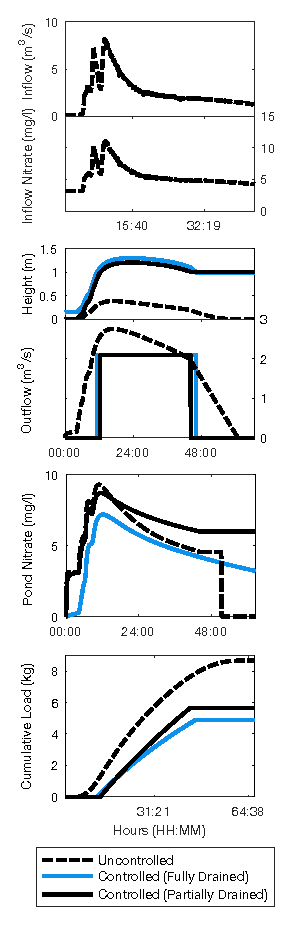
\includegraphics{gfx/Chapter-1/local.eps}
  \caption{Impact of real-time control to hydraulic behavior and nitrate treatment, showing inflow concentrations (top panel), pond water height and outflows (second panel), nitrate concentrations inside the pond (third panel), and cumulative nitrate loads exiting the pond (bottom panel).}\label{fig-ch1:local_control}
\end{figure}

The first case study is motivated by the objective of controlling a single stormwater basin, which was originally designed for flood remediation as a detention pond (flow-through).  The model parameters and physical attributes are provided in the appendix of this chapter. In its original configuration the pond merely serves to attenuate peak flows, with little emphasis on water quality. By equipping this pond with a control valve, its original functionality can remain unaffected during large storms by simply keeping the valve open.  Major water quality benefits can arise, however, by controlling this pond during smaller and more frequent events. 

\

When enabled, the control algorithm keeps the valve closed and only opens it if the water height exceeds 1.0 m to prevent the pond from overflowing. As a further constraint, when the height exceeds 1.0 m the valve is modulated to ensure that outflows do not exceed $2m^3s^{-1}$, which is the threshold at which downstream sediments are assumed to be re-suspended. Two variations of the control algorithm are also evaluated. The first strategy completely drains the pond before a rain event, thus maximizing captured volumes. Based on the magnitude of the rain event (assumed to be known through a weather forecast), the second strategy only partially drains the pond, maximizing the anaerobic conditions at the soil-water interface and thus speeding up denitrification of the inflows. In this case study, the  height of the partially drained configuration was set to 0.15 m, assuming that this height would be sufficient to maintain the saturated conditions and prevent the diffusion of oxygen into soil~\cite{Reddy1989Nitrification-DenitrificationWetlands}. 

\

Compared to the uncontrolled scenario, which only attenuated the peak flow, both
controlled scenarios retained a water height of 1.0 m after the storm
(Figure.\ref{fig-ch1:local_control}). Since the pond can be drained at a later time,
this volume of water was effectively removed from downstream infrastructure
during the storm event.  In static stormwater systems, volume reductions
strategies are typically only assumed to be possible through upstream
infiltration and capture. As such, control may effectively serve as a volume
reduction strategy by shifting flows outside of the storm window. Furthermore,
outflows for the controlled scenarios resembled a ``step'', which kept flows below a predetermined erosion threshold. This reduces downstream sediment loads, compared to the uncontrolled scenario, whose outflows spent over 50\% of the time exceeding the $2~m^3/s$ erosion threshold. 

\

Nitrate inside the pond and the effluent revealed distinct dynamics between each
control configuration. In the uncontrolled scenario, very limited treatment was
present due to short hydraulic retention time. The effluent concentrations
peaked before dropping to zero since the pond drained completely following the
storm. The controlled scenarios did not see this drop-off in internal nitrate
because the flows were retained for treatment. The partially-drained scenario
showed lower nitrate concentrations at the beginning of the storm due higher
anaerobic
soil area and denitrification potential.

\

While internal concentrations are an indicator of treatment dynamics inside the pond, perhaps the best measure of treatment capacity is given by the cumulative nitrate load exiting the pond (bottom panel, figure.\ref{fig-ch1:local_control}). The uncontrolled scenario exhibited the largest cumulative nitrate loads since the runoff effectively just flowed through pond with limited treatment. The controlled pond showed a nearly 43\% mass reduction (from 8.6 kg to 4.9 kg) in nitrate due to increased volume capture, HRT and denitrification. The partially-drained control strategy did indicate an improved load reduction compared to the fully-drained controlled (14\% improvement). This suggests that, rather than simply draining the pond before storm even, improved load reductions may be achieved through more complex control approaches. More complex control comes at the cost uncertainty however. The partially-drained controller assumed prior knowledge about inflows to decide how much water to drain before a storm. If these decisions are made around weather forecasts, the uncertainty embedded in the inputs may cause adverse impacts, such as overflows. The anticipated benefits of any control strategy should thus always be weighted against the uncertainty of any inputs. 


%--------------------------- SYSTEM CONTROL -----------------

\subsection{Case Study 2: System-level Control}

The second case study evaluated how control strategies may change when a system of multiple stormwater assets is controlled. 
A system of four elements was considered, consisting of three parallel ponds draining into a constructed wetland.  (Figure.\ref{fig-ch1:sys_diagram}). 
Two of the upstream ponds were controlled while the treatment wetland and the other pond remained uncontrolled. 
The objective was to control the upstream ponds to boost the nitrate treatment and reduce the effluent concentrations at the outlet of the wetland. 
The configuration was based on a real-world site currently being retrofitted for control in southeastern Michigan. 

\

\begin{figure}
\centering
 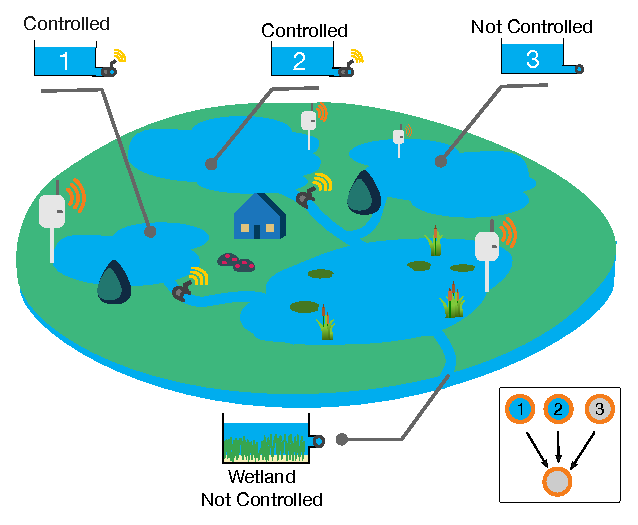
\includegraphics{gfx/Chapter-1/Glo_sys_rep.eps}
 \caption{System-level control case study: three ponds, two of which are controlled, draining into a treatment wetland.}\label{fig-ch1:sys_diagram}
\end{figure}

\begin{figure*}
	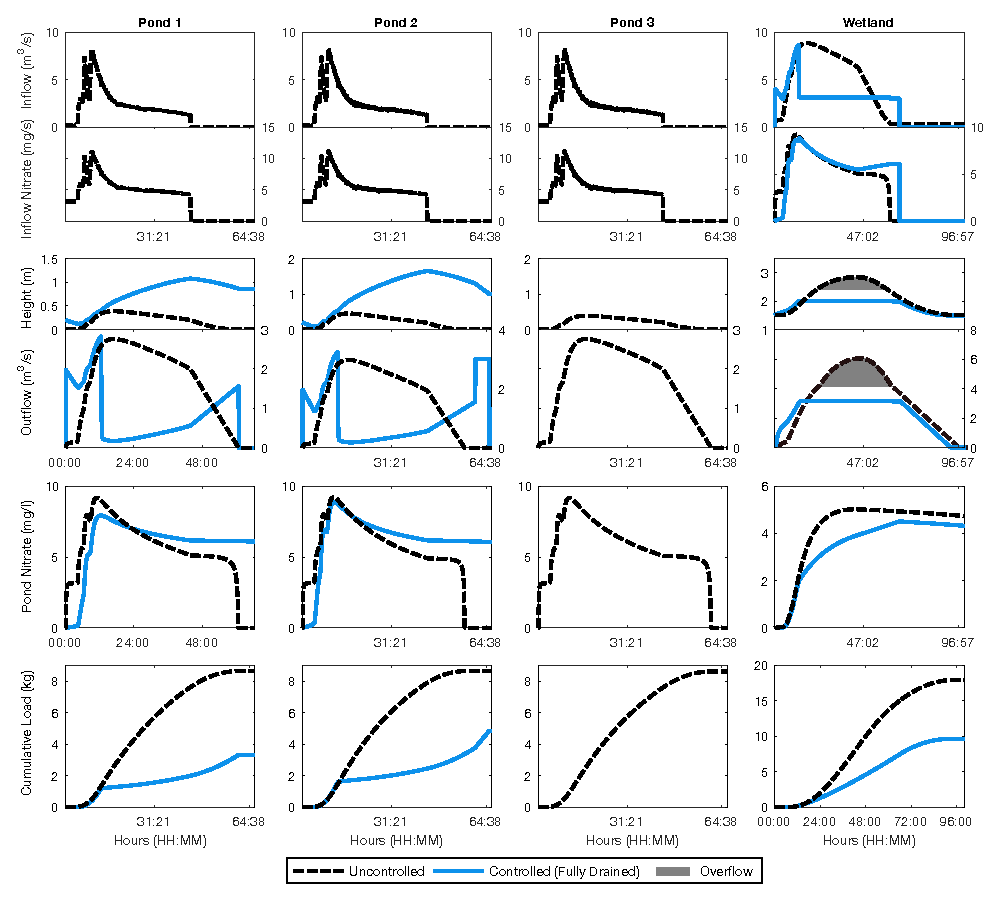
\includegraphics[width=\linewidth]{gfx/Chapter-1/Global.eps}
  \caption{Impact of real-time control to hydraulics and nitrate treatment across a system of stromwater elements: inflow concentrations (top row), pond water height and outflows (second row), nitrate concentrations inside each element (third row), and cumulative nitrate loads exiting the pond (bottom row).}\label{fig-ch1:globalcase}
\end{figure*}

Due to their large biomass area, wetlands have a higher nitrate treatment capacity than ponds\cite{Scholes2008APotentials}. 
As such, the control objective was to keep the downstream wetland ``active'', by
maximizing its water height and thus the biomass treatment area. While a prolonged  inundation may damage the emergent vegetation in the wetland, the proposed control algorithm maximizes the treatment area of wetland only during the duration of the storm event, which should improve the treatment while only briefly inundating the wetland.
In the uncontrolled scenario the flows from the upstream ponds actually added up to cause the wetland to overflow (Figure.~\ref{fig-ch1:globalcase}, fourth column), which also impaired treatment. 

\

The controlled scenario (see appendix for implementation details) balanced the outflows from the two ponds to ensure that the wetland remained filled (2 m --- just below its overflow height) as long as the uncontrolled third pond was discharging. Once the third pond was entirely drained, the upstream ponds retained any additional inflows, as long as it would not cause them to overflow. This strategy eliminated downstream overflows while simultaneously increasing the wetland's anaerobic treatment area. As such, flows from the third pond were exposed to a larger denitrification than in the uncontrolled case. Overall, the controlled system achieved a 46.48\% (from 17.9 kg to 9.6 kg) reduction in cumulative nitrate loads.  While some of this overall reduction was driven by the fact that the two controlled ponds remained filled after the storm, thus retaining some nitrate mass upstream, two major benefits arose compared to the uncontrolled scenario. Firstly, the wetland effluent concentrations were reduced over time, showing a 15.25\% reduction in concentration. Secondly, the case study showed that a subset upstream elements may be controlled to reduce downstream hydraulic loads, which, similar to the first case study, has the potential to reduce erosion. 

\

A natural extension of this control strategy would be the direct control of the wetland. In many real-world situations, however, not all elements of the system will be controllable. In these instances, system-level benefits may still be achieved via control of other elements. The purpose of this case study was to illustrate one possible example focused on system-level nutrient control. While simple, this control strategy was nonetheless effective at improving the hydraulic and water quality behavior of the overall system. More complex control strategies will be evaluated in the future, especially in the context of larger and more heterogeneous stormwater systems. 


%--------------------------- Discussion -----------------
\begin{figure*}
\centering
\includegraphics[width=.9\textwidth]{gfx/Chapter-1/arch.png}
  \caption{The stormwater \textit{feedback control loop}. A desired watershed outcome is compared, in real-time, to actual watershed state based on sensor measurements. The control logic then adjusts the states of valves, gates and pumps to drive the system toward the desired state. Disturbances, such as precipitation, may drive the system away from the desired outcome and must be controlled against when the feedback loop repeats.}\label{fig-ch1:rsch_gaps}
\end{figure*}

\section{Discussion}
Sensor-driven, real-time control of stormwater presents an exciting new paradigm and research area. It is presently unclear, however, how results generated by existing research, as well as the case studies presented in this chapter, can be scaled to large watersheds. 
Many existing studies focus solely on the control of individual elements and, specifically, on sediment reduction or flood remediation. 
While the case studies in this chapter took a step toward simulating the removal of more complex dissolved pollutants in a multi-element system, it is important to note that the control logic was uniquely  tailored to one specific storm and study area. 
The efficacy of the controls in our case studies was reliant on the ability to hold water after a storm to allow for extended treatment. 
This strategy may be impacted by limits on hydraulic retention time.
Modifying the water levels and residence times, may introduce issues related to aesthetics, plant survival and mosquito breeding\cite{Knight2003211}. Thus, the potential benefits to water flow and quality must studied as part of a mutli-objective optimization problem.

\

Much of the real word is underpinned by significant uncertainty, especially related to weather forecasts. 
Since these forecasts determine when and how much water needs to be released, the stochastic nature of weather must be taken into consideration when controlling such systems. 

Control strategies may also change entirely if the removal of different pollutants is required. 
A simple example can be given by watersheds in which runoff is dominated by ammonia rather than nitrate, thus requiring stages of both nitrification and denitrification. 
The intricacy of control strategies will likely increase with the
  number of objectives\cite{Tillinghast_2012} and the complexity of runoff dynamics. This introduces the exciting paradigm of controlling the overall system to create treatment chains in which individual elements are tuned to achieve specific objectives. 
By tuning the hydraulic behavior of each element, there will be an unprecedented opportunity to begin applying process-based knowledge from wastewater treatment to distributed stormwater modeling. 
The modeling of such complete control approaches will be made easier by the simulation approach proposed in Figure.\ref{fig-ch1:framework}, which will permit for coupling of knowledge spanning hydrology, hydraulics, and water quality.  


\section{Knowledge gaps}
While research is needed to improve our fundamental understanding and modeling of system-level stormwater, two major knowledge gaps become evident when we view stormwater control in a system-theoretic framework. This can be accomplished by visualizing it as a \textit{feedback loop} (Figure~\ref{fig-ch1:rsch_gaps}), a technique common in the control communities and dynamical systems theory\cite{Ogata201}. This loop estimates the difference between a desired watershed outcome (downstream nitrate concentrations, for example) and the actual watershed outcome and \textit{feeds} it into control logic to drive the system toward the desired outcome. The physical requirements of this feedback loop, which include sensors, controllers and the physical infrastructure already exist or have matured to the point at which they  do not present a major research challenges. Rather, our biggest knowledge gaps span the \textit{virtual} components of the feedback loop and include the (1) assimilation of noisy, sparse, and heterogeneous sensor data into real-time models (state estimation), and (2) the automated synthesis of control logic in response to these estimates. 

\subsection{Toward a new generation of real-time models}
Unlike in static infrastructure systems, where adaptation strategies take place on monthly or yearly times scales, real-time control reduces adaptation to minutes or seconds. Existing stormwater models have not been designed to interface with real-time data. Rather, sensor data is often used merely as a convenience to parameterize the model. It is not uncommon for these predictions to drift away from real-world conditions over the modeling horizon. Given the need to base control actions on the best sources of information, a new generation of data-driven and real-time models must be developed. Rather than executing unchecked into the future, they will ``learn'' from the data and update their states to reflect changing field conditions. Such models will need to be self-calibrating, robust to uncertainty, and computationally efficient to execute in the amount of time required to make control decisions. This raises the question: how complex does a system model need to be to enable an effective and robust control loop? While the answer to this question remains to be investigated, many other control applications (aircraft autopilots, for example) suggest that it is very likely that stormwater control models will not need to be as complex as the models currently used for simulation. This does not mean that existing physically-driven models or our proposed simulation framework (figure~\ref{fig-ch1:framework}) will not be needed. In fact, existing simulations approaches will be critical in the planning and design of control systems, while real-time models will be used for the actual control.

\

In our case studies an assumption was made that control actions were informed by known in-situ conditions, such as water flows, pond levels, and nitrate concentrations. This will be far from true in many real-world control systems, where sensors will be sparsely placed and noisy. New models will thus have to be developed to make predictions at locations that are uninstrumented and for parameters that are unmeasured.  By quantifying the uncertainty inherent in such models, it will also be possible to develop sensor placement algorithms to determine how many sensors are required and where they should be placed to improve real-time model performance. Many of the methods required for these tasks already exist in other communities (system identification, data assimilation, machine learning, etc), but their application to stormwater systems remains to be investigated.


\subsection{Control Algorithms}
Presently, it is unclear which real-time control and optimization techniques will be the most robust and suitable for distributed stormwater systems.  Most current studies, as well as the case studies presented in this chapter, have been built around simple rule-based control (e.g.\ drain a pond before a storm). While such control approaches preserve intuition and incorporate operator expertise, the approach does not scale for systems of arbitrary sizes. This impedes the ability to transfer lessons from one watershed to another. The complexity of operational rules will increase drastically with the size of a watersheds or extended control objectives. The logic associated with operating a network of distributed stormwater assets, comprised of hundreds or thousands of controllers, will become overwhelming unless formal mathematical methods are developed to abstract the physical stormwater dynamics into a system-theoretic framework. These mathematical underpinnings will finally allow for performance or safety guarantees to be provided. This, in turn, will enable new methods to determine how many controllers are needed and where they should be placed to ensure that desired watershed outcomes are met. 

\section{Conclusions}
The goal of this chapter was to illustrate the need for a ``smart'' stormwater systems theoretical framework. Before such systems become adopted, much work remains to be conducted on simulating their performance, which can be accomplished by coupling existing hydrologic, hydraulic and water quality models. As demonstrated by our case studies, real-time control of stormwater has the potential to significantly improve the performance of existing infrastructure, introducing new alternatives to tightly manage nutrients, metals and other pollutants in urban watersheds. Considering current funding mechanisms for stormwater, especially in the United States, the cost of retrofitting will provide a more budget-conscious alternative to new construction while achieving similar or better water quality outcomes. Aside from technical or research gaps, which must be addressed before these systems become reality, it will be imperative to encourage a broad community of researchers, engineers, and cities to adopt these technologies as part of their existing toolboxes. To that end, our team has been spearheading the \href{http://open-storm.org}{open-storm.org} portal, a collaborative and open-source initiative aimed at sharing end-to-end blueprints and tutorials on software, hardware and sensors required to instrument and control urban watersheds. As the community grows around this exciting new area of research, \href{http://open-storm.org}{open-storm.org} will track and disseminate its future work.
